\documentclass[a4paper,12pt]{report}
\usepackage[utf8]{inputenc}
\usepackage[left=1.25in, right=1.25in]{geometry}
\usepackage{graphicx}
\usepackage{titlesec}
\usepackage{adjustbox}
\usepackage{epigraph}
\usepackage{listings}
\usepackage{xcolor}

\definecolor{lightgray}{rgb}{0.97,0.97,0.97}
\definecolor{darkgreen}{rgb}{0.2,0.5,0.2}
\definecolor{darkred}{rgb}{0.64,0.09,0.09}
\lstset{ 
	backgroundcolor=\color{lightgray},
	basicstyle=\fontsize{8}{12}\ttfamily,
	breakatwhitespace=false,
	breaklines=true,
	captionpos=b,,
	escapeinside={\%*}{*)},
	extendedchars=true,
	commentstyle=\color{blue},
	frame=single,
	keepspaces=true,
	keywordstyle=\color{darkred},
	language=SQL,
	morekeywords={GROUP\_CONCAT, FILTER, OPTIONAL, BIND, BOUND},
	deletekeywords={KEY,YEAR,ELSE},
	numbers=none,
	rulecolor=\color{gray},
	showspaces=false,
	showstringspaces=false,
	showtabs=false,
	stepnumber=2,
	stringstyle=\color{darkgreen},
	tabsize=2
}

\graphicspath{ {images/} }
\setlength\epigraphwidth{0.7\textwidth}

\title{Developing a virtual assistant for answering music related questions}
\author{Claudio SCALZO \and Luca LOMBARDO}

\begin{document}
\maketitle
\tableofcontents

\chapter{Introduction}
	\section{Why a virtual assistant?}
	\section{Scope of the project}
	\section{Expected results}

\chapter{Natural Language Understanding}
	\section{What is NLU?}
	\section{How it works? (Papers)}
	\section{State of art}

\chapter{Dialogflow}
	\section{What is Dialogflow}
	\section{Why Dialogflow}
	\section{How it works?}

\chapter{DOREMUS}
	\section{What is DOREMUS}
	\section{How is organized}
	\section{How to integrate it in our project}

\chapter{The bot}
	\section{The architecture}
	The architecture of the bot is divided in four categories:
	\begin{center}
		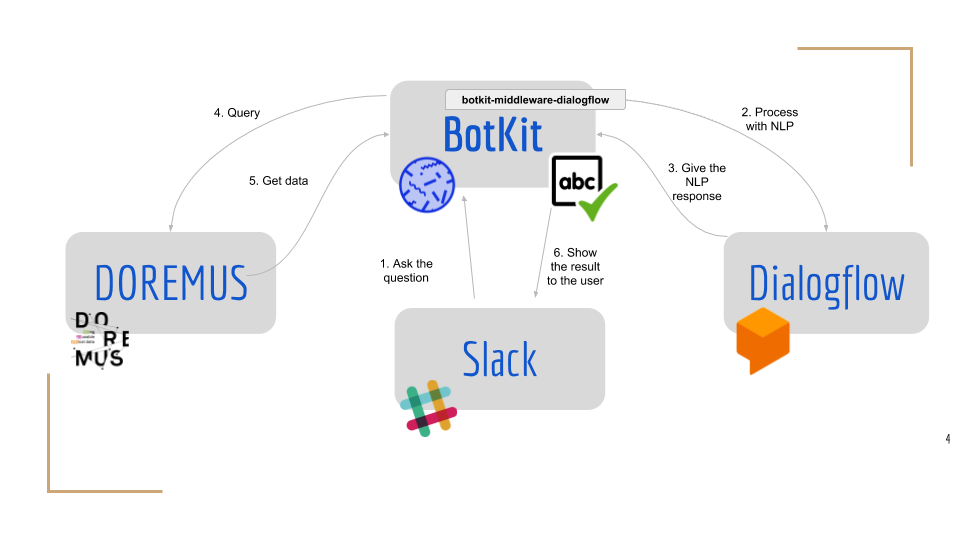
\includegraphics[scale=0.4]{architecture}
	\end{center}
	First of all we can find the client, that in the case of our development, testing and validation process, has been \textit{Slack}. Of course, it can be any of the clients which support the installation of the bot on it (\textit{Telegram}, \textit{Facebook Messenger}, etc.). The use of Slack let us to exploit the beautiful \textit{Slack Cards}, to make the answers of our bot (works, artists, performances) prettier and easier to understand in a glance. A set of examples will be provided in the last chapter.\\\\
	The second part of the architecture is represented by the NLP. In this case, as told in the previous chapter, we used \textit{Dialogflow}, to exploit its advanced slot-filling techniques and its NLU power.\\\\
	However, we didn't use \textit{Dialogflow} on its own, exploiting the direct integration with \textit{Slack}, but we used something that we placed in the middle of the two: \textit{BotKit}. \textit{BotKit} is a bot-making toolkit that aims to ease the building process of a bot, potentially exploiting different NLPs and/or different clients. In our case, \textit{BotKit} has been deployed on a web server, and thanks to the \textit{NodeJS} code we were able to come up with a series of features (like the spell checker) that would have been impossible to reach with a simple (direct) integration between \textit{Slack} and \textit{Dialogflow}. We'll talk more about that in the following paragraphs.\\\\
	The last part of the architecture is of course represented by the data source: \textit{DOREMUS}. We talked about that in the previous chapters, but from the architecture is important to notice how the knowledge base is queried: each query is dynamic, in the sense that according to the intent, the number of filters and the desired results wanted by the user, the query will have a different shape and a different content. The code in the web server is able to add different pieces of queries according to what \textit{Dialogflow} is able to understand and to provide as output values of the API.\\\\
	
	\section{Entities}
	The sentences that the bot is required to recognize are of course full of informations related to the \textit{DOREMUS} knowledge base. This means that the NLP has to be able to understand some "entities" (informations, words, piece of sentences) that are not in the standard language, but are related to the \textit{DOREMUS} or, in general, musical world. Our bot is equipped with three different entities:
	\begin{itemize}
		\item \texttt{doremus-artist}\\
		Contains all the artists in the \textit{DOREMUS} knowledge base. It's organized in a \textit{key-value} pair where the \textit{key} is the unique id of the artist inside the knowledge base, and the \textit{value} is the set of full names and surnames of the artist, in all the available language of the knowledge base.
		The query with which the artist were retrieved is the following:
		\begin{lstlisting}

		SELECT DISTINCT ?composer
		  (GROUP_CONCAT (DISTINCT ?name; separator="|") AS ?names)
		  (GROUP_CONCAT (DISTINCT ?surname; separator="|") AS ?surnames)
		  (COUNT (?expression) AS ?count)
		WHERE {
		  ?expression a efrbroo:F22_Self-Contained_Expression .
		  ?expCreation efrbroo:R17_created ?expression ;
		    ecrm:P9_consists_of / ecrm:P14_carried_out_by ?composer .
		  ?composer foaf:name ?name .
		  ?composer foaf:surname ?surname 
		}
		GROUP BY ?composer
		ORDER BY DESC (?count)
		\end{lstlisting}
		The artists are ordered by descending count of works, in order to have the most famous artists at the top of the entity dictionary, and let \textit{Dialogflow} find the most famous artists in case just a surname is given. The result of the query has been taken as a \texttt{.csv} file and then processed a little bit (delete the count, join the names and surnames columns, duplicate the composer id, eliminate the pipes and some special characters) in order to fit with the \textit{Dialogflow}'s constraints.
		
		\item \texttt{doremus-instrument}\\
		Contains all the instruments of the \texttt{iaml/mop/} dictionary of the \textit{DOREMUS} knowledge base. Also in this case the \textit{key-value} pair dictionary has as keys the id of the instrument, and as values all the synonyms (names in different languages). The query thanks to which we retrieved this entity is:
		\begin{lstlisting}
		
		SELECT DISTINCT ?instrument
		  (GROUP_CONCAT (DISTINCT ?instrument; separator="|") AS ?instruments)
		WHERE {
		  ?instr skos:prefLabel ?instrument .
		  ?instr skos:topConceptOf | skos:inScheme ?res .
		  VALUES (?res) {
		    (<http://data.doremus.org/vocabulary/iaml/mop/>)
		  }
		}
		GROUP BY ?instr
		\end{lstlisting}
		
		\item \texttt{doremus-genre}\\
		Contains all the genres of the \texttt{iaml/genre/} dictionary of the \textit{DOREMUS} knowledge base. The query thanks to which we retrieved this entity is:
		\begin{lstlisting}
		
		SELECT DISTINCT ?gen
		(GROUP_CONCAT (DISTINCT ?genre; separator="|") AS ?genres)
		WHERE {
		  ?gen skos:prefLabel ?genre .
		  ?gen skos:topConceptOf | skos:inScheme ?res .
		  VALUES (?res) {
		    (<http://data.doremus.org/vocabulary/iaml/genre/>)
		  }
		}
		GROUP BY ?gen
		\end{lstlisting}
	\end{itemize}

	\section{Intents}
	The intents are grouped in a simple and clear way, according to what the user wants to retrieve from the \textit{DOREMUS} knowledge base:
	\begin{itemize}
		\item \texttt{works-by}\\
		Retrieves a set of works according to different filters (artists who composed the works, instruments used, music genre and/or year of composition).
		\item \texttt{find-artist}\\
		Finds a set of artists according to some filters (number of composed works, number of works of a given genre, etc.).
		\item \texttt{find-performance}\\
		Propose to the user a future performance (that can be filtered by city and/or date period), or shows to the user the details of a past performance.
		\item \texttt{discover-artist}\\
		Shows a card with a summary of an artist, with its birth/death place and date, a picture and a little bio. After the card visualization, a set of works of the artist (connection with the \texttt{works-by} intent) can be asked.
	\end{itemize}
	Now we're going to go deeper in the intent descriptions.
	\subsection{Retrieving a set of works}
	The \texttt{works-by} intent is the most complex one in the entire bot's intents set. It can retrieve a certain number of works from 1 to \textit{L}, where \textit{L} is the number specified by the user if it's smaller than the number of available works. Otherwise, if it's greater, all the avilable works are returned. Its default value (if not specified by the user) is 5.\\\\
	The filters can be various:
	\begin{itemize}
		\item \textbf{Artist:}
		the artist name (full or surname).\\
		\textit{"Give me 3 works composed by Bach"}
		
		\item \textbf{Instruments:}
		the instrument(s) (in \texttt{and}/\texttt{or} relation).\\
		\textit{"Give me 2 works for violin, clarinet and piano"}\\
		\textit{"Tell us 4 works for violin or piano"}
		
		\item \textbf{Genre:}
		the music genre.\\
		\textit{"List me 10 works of genre concerto"}
		
		\item \textbf{Composition period:}
		the period in which the work has been written.\\
		\textit{"Tell me one work composed during 1811"}\\
		\textit{"Give us 3 works written between 1782 and 1821"}
		
	\end{itemize}
	The filters can be specified in every way: this means that the user can specify all the available filters, some of them and even none. If the number of filters in the first query is smaller than two, the bot asks the user if he wants to apply other filters. The user can answer positively or negatively, and then decide which kind of filter (and the value) to apply. It's important to notice that the kind of filter and the value can be specified together or not; let's see an example to make it more clear.\\\\
	First of all, we are in the context in which the bot asks the users if he wants to apply some filters:
	
	\begin{verse}
	\textit{Please give me 3 works by Beethoven!} - \textbf{User}\\
	\textit{You told me few filters. Do you want to add something?} - \textbf{Bot}\\
	\textit{Yes!} - \textbf{User}\\
	\textit{Ok, tell me what} - \textbf{Bot}\\
	\end{verse}
	In this case, two scenarios can happen:
	\begin{verse}
	\textit{The composition year} - \textbf{User}\\
	\textit{Of course! Tell me the time period.} - \textbf{Bot}\\
	\textit{Between 1787 and 1812} - \textbf{User}\\
	\end{verse}
	or directly...
	\begin{verse}
	\textit{Only works composed between 1787 and 1812} - \textbf{User}\\
	\end{verse}
	The \textbf{dynamic} query used for the works by artist intent is the following:
	\begin{lstlisting}
	
	SELECT DISTINCT ?title, ?artist, year(?comp) AS ?year, ?genre, ?comment, ?key
	WHERE {
	
		------------------------------------------------------------ STATIC SECTION
		?expression a efrbroo:F22_Self-Contained_Expression ;
		  rdfs:label ?title ;
		  rdfs:comment ?comment ;
		  mus:U13_has_casting ?casting ;
		  mus:U12_has_genre ?gen .
		?expCreation efrbroo:R17_created ?expression ;
		  ecrm:P4_has_time-span ?ts ;
		  ecrm:P9_consists_of / ecrm:P14_carried_out_by ?composer .
		?composer foaf:name ?artist .
		?gen skos:prefLabel ?genre .
		?ts time:hasEnd / time:inXSDDate ?comp .
		OPTIONAL {
			?expression mus:U11_has_key ?k .
			?k skos:prefLabel ?key
		} .
		
		------------------------------------------------------------ DYNAMIC SECTION
		
		------------- Instrument
		?casting mus:U23_has_casting_detail ?castingDetail .
		?castingDetail mus:U2_foresees_use_of_medium_of_performance
		               / skos:exactMatch* ?instrument .
		VALUES(?instrument) {
		  (<http://data.doremus.org/vocabulary/iaml/mop/' + instrument + '>)
		}
		
		------------- Genre
		VALUES(?gen) {
		  (<http://data.doremus.org/vocabulary/iaml/genre/' + genre + '>)
		}
		
		------------- Artist
		VALUES(?composer) {
		  (<http://data.doremus.org/artist/' + artist + '>)
		}
		
		------------- Composition Year
		FILTER (?comp >= "' + yearstart + '"^^xsd:gYear AND
		        ?comp <= "' + yearend + '"^^xsd:gYear)
	}
	ORDER BY rand()
	LIMIT ' + num '
	\end{lstlisting}
	It's important to notice the particularity of the instrument information because, as previously said, it can be a list of instrument connected by an \texttt{and/or} logic operator. In the query implemented inside the \texttt{works-by} intent, this doesn't mean only to create dynamically the query (like for the other informations) but also to differentiate the code between a single-instrument filter, an "and" multi-instrument filter and an "or" multi-instrument filter. The differences are shown here:
	\begin{lstlisting}
	
	---- AND CASE
	if (strictly === "and") {
	  for (var i = 0; i < instr.length; i++) {
	    query += '?casting mus:U23_has_casting_detail ?castingDetail' + i + ' .
	            ?castingDetail' + i + '
	              mus:U2_foresees_use_of_medium_of_performance
	              / skos:exactMatch* ?instr' + i + ' .
	            VALUES(?instr' + i + ') {
	              (<http://data.doremus.org/vocabulary/iaml/mop/' + instr[i] + '>)
	            }'
	  }
	}
	
	---- OR CASE
	else {
	  query += '?casting mus:U23_has_casting_detail ?castingDetail .
	            ?castingDetail
	              mus:U2_foresees_use_of_medium_of_performance
	              / skos:exactMatch* ?instr .
	            VALUES(?instr) {'
	
	  for (var i = 0; i < instr.length; i++) {
	    query += '(<http://data.doremus.org/vocabulary/iaml/mop/' +instr[i] + '>)'
	  }
	}
	\end{lstlisting}
	In the \texttt{and} case we add (with a \texttt{for} operator that loops through the \texttt{instr} array) a \texttt{castingDetail} for each instrument, forcing its value to that specific instrument. In the \texttt{or} case, instead, the \texttt{castingDetail} is just one and can assume a set of values filled with the \texttt{for} operator that loops through the \texttt{instr} array. 

	\subsection{Finding some artists}
	\subsection{Finding some future and past performances}
	The bot is also capable of giving the user some future and past performances and events. The place and the time period can be, of course, specified in the query. The query is the following:
	\begin{lstlisting}
	
	SELECT ?title, ?subtitle, ?actorsName, ?placeName, ?date
	WHERE {
	  ?performance a mus:M26_Foreseen_Performance ;
	    ecrm:P102_has_title ?title ;
	    ecrm:P69_has_association_with / mus:U6_foresees_actor ?actors ;
	    mus:U67_has_subtitle ?subtitle ;
	    mus:U7_foresees_place_at ?place ;
	    mus:U8_foresees_time_span ?ts .
	  ?place rdfs:label ?placeName .
	  ?actors rdfs:label ?actorsName .
	  ?ts time:hasBeginning / time:inXSDDate ?time ;
 	    rdfs:label ?date .
	  FILTER ( ?time >= "' + startdate + '"^^xsd:date AND
	           ?time <= "' + enddate + '"^^xsd:date ) .
	  FILTER ( contains(lcase(str(?placeName)), "' + city + '") )
	}
	ORDER BY rand()
	LIMIT ' + number '
	\end{lstlisting}
	And here there is an example:
	\begin{verse}
		\textit{Tell me one event in Paris!} - \textbf{User}\\
		\textit{In which period?} - \textbf{Bot}\\
		\textit{Next month} - \textbf{User}\\
	\end{verse}
	\subsection{Know more about an artist}
	The last intent of the bot is \texttt{discover-artist}. This is the richest intent in terms of informations provided: it returns the artist summary in a \textit{Slack card}, with a picture, a short bio, the birth/date places and dates.
	The query is the following:
	\begin{lstlisting}
	
	SELECT DISTINCT ?composer, ?name, ?bio, xsd:date(?d_date) as ?death_date,
	                ?death_place, xsd:date(?b_date) as ?birth_date, ?birth_place, ?image
	WHERE {
	  VALUES(?composer) {(<http://data.doremus.org/artist/' + artist + '>)} .
	  ?composer rdfs:comment ?bio .
	  ?composer foaf:depiction ?image .
	  ?composer schema:deathDate ?d_date .
	  ?composer foaf:name ?name .
	  ?composer dbpprop:deathPlace ?d_place .
	  OPTIONAL { ?d_place rdfs:label ?death_place } .
	  ?composer schema:birthDate ?b_date .
	  ?composer dbpprop:birthPlace ?b_place .
	  OPTIONAL { ?b_place rdfs:label ?birth_place } .
	  FILTER (lang(?bio) = "en")
	}
	\end{lstlisting}
	And here there is an example:
	\begin{verse}
		\textit{Tell me something about Mozart} - \textbf{User}\\
	\end{verse}
	or...
	\begin{verse}
		\textit{What do you know about Beethoven?} - \textbf{User}\\
	\end{verse}

	\section{The flow}
	\section{The spell checker}
	
\end{document}          
